\subsection{Decisor}
\paragraph{}
\begin{figure}[h]
  \begin{center}
  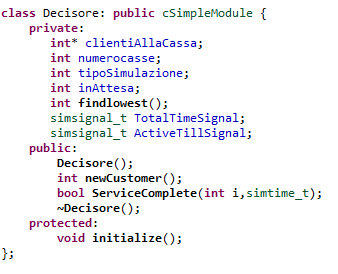
\includegraphics[width=80mm]{decisore.png}
  \caption{Decisor.}
  \label{fig:dec}
  \end{center}
\end{figure}
The decisor is an entity that chooses, using a "random" definible algorithm the till in which switch the customer. Its structure is shown in figure \ref{fig:dec}.
The functions that make up the decisor are the following: 
\paragraph{findlowest}
This function is used to find which till has the tie with the minimum number of people who are waiting to be served. At the beginning we check the parameter who indicates the type of simulation we want to execute: ties with a common queue (case 1) or ties with own queue (case 2). The function has input parameter: parametro(int), that is used to define which case we are simulating and an output: int that represents the index of the tie with the minimum number of element in queue, and if the ties have only one element, the first free tie. If two or more ties have the same elements in queue, the function chooses the till with the lowest index.
\paragraph{newCustomers}
This function finds the right till for the new customer; once it was found it must add the specific time-delay, because we want to simulate the time to reach the till, and only after that time is elapsed our new customer is added to the queue.
The function has an input parameter: parameter(int) that is used to define which case we are simulating and an output: int that return the position of the till.
\paragraph{ServiceComplete}
This method is used by the till to indicate that it has finished serving one customer, and in particular is usefull in case of a common queue, because the till are work-conserving, i.e. all customers in queue must be served without going in idle. This function is called by a till when it has served a customer and if there are other customers in queue it assign the first of them immediately to the till who has called this method.
